\documentclass{article}
\usepackage[utf8]{inputenc}
\usepackage{amsmath}
\usepackage{amsthm,amssymb}
\usepackage[dvipsnames]{xcolor}
\usepackage{tikz}
\usetikzlibrary{arrows.meta, bending}
\usetikzlibrary{matrix, positioning}

\begin{document}

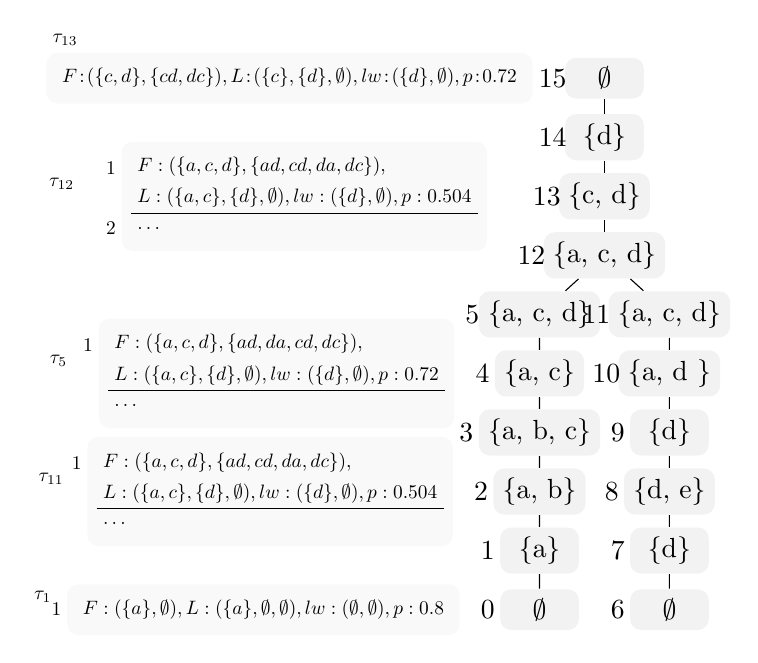
\begin{tikzpicture}[scale = 0.75, node/.style={rectangle, rounded corners, minimum width=1cm, fill=lightgray!20}]

    \node[node] (15) at (0, 0) {$\emptyset$};
    \node[node] (14) at (0,-1) { \{d\}};
    \node[node] (13) at (0,-2) {\{c, d\}};
    \node[node] (12) at (0,-3) {\{a, c, d\}};

    \node[node] (5) at (-1.1,-4) {\{a, c, d\}};
    \node[node] (4) at (-1.1,-5) {\{a, c\}};
    \node[node] (3) at (-1.1,-6) {\{a, b, c\}};
    \node[node] (2) at (-1.1,-7) {\{a, b\}};
    \node[node] (1) at (-1.1,-8) {\{a\}};
    \node[node] (0) at (-1.1,-9) {$\emptyset$};

    \node[node] (11) at (1.1,-4) {\{a, c, d\}};
    \node[node] (10) at (1.1,-5) {\{a, d \}};
    \node[node] (9) at (1.1,-6) {\{d\}};
    \node[node] (8) at (1.1,-7) {\{d, e\}};
    \node[node] (7) at (1.1,-8) {\{d\}};
    \node[node] (6) at (1.1,-9) {$\emptyset$};     

    \draw (0) -- (1);
    \draw (1) -- (2);
    \draw (2) -- (3);
    \draw (3) -- (4);
    \draw (4) -- (5);
    \draw (5) -- (12);
    \draw (6) -- (7);
    \draw (7) -- (8);
    \draw (8) -- (9);
    \draw (9) -- (10);
    \draw (10) -- (11);
    \draw (11) -- (12);
    \draw (12) -- (13);
    \draw (13) -- (14);
    \draw (14) -- (15);
   
   
    \node at ([xshift=-2mm]0.west) {0};
    \node at ([xshift=-2mm]1.west) {1};
    \node at ([xshift=-2mm]2.west) {2};
    \node at ([xshift=-2mm]3.west) {3};
    \node at ([xshift=-2mm]4.west) {4};
    \node at ([xshift=-1mm]5.west) {5};
    \node at ([xshift=-2mm]6.west) {6};
    \node at ([xshift=-2mm]7.west) {7};
    \node at ([xshift=-2mm]8.west) {8};
    \node at ([xshift=-2mm]9.west) {9};
    \node at ([xshift=-2mm]10.west) {10};
    \node at ([xshift=-2mm]11.west) {11};
    \node at ([xshift=-2mm]12.west) {12};
    \node at ([xshift=-2mm]13.west) {13};
    \node at ([xshift=-2mm]14.west) {14};
    \node at ([xshift=-2mm]15.west) {15};


    \matrix (table) [matrix of nodes, nodes in empty cells,
        nodes={ minimum height=5mm, anchor= center, scale =0.7, anchor=west}, rounded corners, row sep=-\pgflinewidth, left = 9mm of 13, fill = lightgray!10] (12-table) {
$F:(\{a,c,d\},\{ad,cd,da,dc\}),$ \\ 
$L:(\{a,c\},\{d\},\emptyset), lw:(\{d\},\emptyset), p:0.504$ \\ \hline
$\dots$ \\
    };
    \foreach \rowIndex [count=\rowNumber from 1] in {1, 3} {
        \node[left=1mm of 12-table-\rowIndex-1.west, anchor=east, scale=0.7] { \rowNumber};
    }
    \node[left=10mm of 12-table.west, anchor=south west, scale=0.7] (title) {$\tau_{12}$};


    \matrix (table) [matrix of nodes, nodes in empty cells,
        nodes={ minimum height=5mm, anchor= center, scale =0.7, anchor=west}, rounded corners, row sep=-\pgflinewidth, left = 5mm of 0, fill = lightgray!10] (1-table) {
         $F:(\{a\},\emptyset), L:(\{a\},\emptyset,\emptyset),lw:(\emptyset,\emptyset), p:0.8$ \\
        };
    \foreach \rowIndex [count=\rowNumber from 1] in {1} {
        \node[left=1mm of 1-table-\rowIndex-1.west, anchor=east, scale=0.7] { \rowNumber};
    }
    \node[left=5mm of 1-table.west, anchor=south west, scale=0.7] (title) {$\tau_{1}$};

    \matrix (table) [matrix of nodes, nodes in empty cells,
        nodes={ minimum height=5mm, anchor= center, scale =0.7, anchor=west}, rounded corners, row sep=-\pgflinewidth, left = 4mm of 15, fill = lightgray!10] (13-table) {

        $F\!:\!(\{c,d\},\{cd,dc\}),L\!:\!(\{c\},\{d\},\emptyset),lw\!:\!(\{d\},\emptyset), p\!:\!0.72$
 \\
        };
    %
    %
    %
    \node[above=0mm of 13-table.north west, anchor=south west, scale=0.7] (title) {$\tau_{13}$};


     \matrix (table) [matrix of nodes, nodes in empty cells,
        nodes={ minimum height=5mm, anchor= center, scale =0.7, anchor=west}, rounded corners, row sep=-\pgflinewidth, left = 5mm of 4, fill = lightgray!10] (5-table) {

        $F:(\{a,c,d\},\{ad,da,cd,dc\})$, \\
       $ L:(\{a,c\},\{d\},\emptyset),lw:(\{d\},\emptyset), p:0.72$ \\ \hline
        \dots \\
        };
    \foreach \rowIndex [count=\rowNumber from 1] in {1} {
        \node[left=1mm of 5-table-\rowIndex-1.west, anchor=east, scale=0.7] { \rowNumber};
    }
    \node[left=7mm of 5-table.west, anchor=south west, scale=0.7] (title) {$\tau_{5}$};


    \matrix (table) [matrix of nodes, nodes in empty cells,
        nodes={ minimum height=5mm, anchor= center, scale =0.7, anchor=west}, rounded corners, row sep=-\pgflinewidth, left = 5mm of 2, fill = lightgray!10] (11-table) {

        $F:(\{a,c,d\},\{ad,cd,da,dc\}),$ \\ 
$L:(\{a,c\},\{d\},\emptyset), lw:(\{d\},\emptyset), p:0.504$ \\ \hline

\dots \\
        };
    \foreach \rowIndex [count=\rowNumber from 1] in {1} {
        \node[left=1mm of 11-table-\rowIndex-1.west, anchor=east, scale=0.7] { \rowNumber};
    }
    \node[left=7mm of 11-table.west, anchor=south west, scale=0.7] (title) {$\tau_{11}$};

\end{tikzpicture}

\end{document}